\documentclass[a4paper]{article}
\usepackage{amssymb}
\usepackage{gensymb}
\usepackage{mhchem}
\usepackage{parskip}
\usepackage{multirow}
\usepackage{caption}
\usepackage{graphicx}
\usepackage[
    a4paper,
    left=32mm,
    right=32mm,
    top=40mm,
    bottom=32mm
]{geometry}
\usepackage[T1]{fontenc}
\usepackage[ngerman]{babel}

\graphicspath{ {../} }

% \setlength{\parindent}{0pt}
\renewcommand{\arraystretch}{1.2}

\begin{document}
\section*{Protokoll}
\subsection*{Geräte und Chemikalien}
\begin{tabular}{|l|c|}
    \hline
    Gerät & Anzahl \\
    \hline
    Becherglas & 4 \\
    Krokodilklemme & 2 \\
    Kabel & 2 \\
    Voltmeter & 1 \\
    Filterpapier & 1 \\
    \hline
\end{tabular}

\begin{tabular}{|l|}
    \hline
    Chemikalie \\
    \hline
    \ce{ZnSO4_{(aq)}} \\
    \ce{CuSO4_{(aq)}} \\
    \ce{AgNO3_{(aq)}} \\
    \ce{FeSO4_{(aq)}} \\
    \ce{Zn}-Blech \\
    \ce{Cu}-Blech \\
    \ce{Ag}-Blech \\
    \ce{Fe}-Blech \\
    \ce{KNO3}-Lösung \\
    \hline
\end{tabular}

\subsection*{Durchführung}

\begin{figure*}[h]
    \centering
    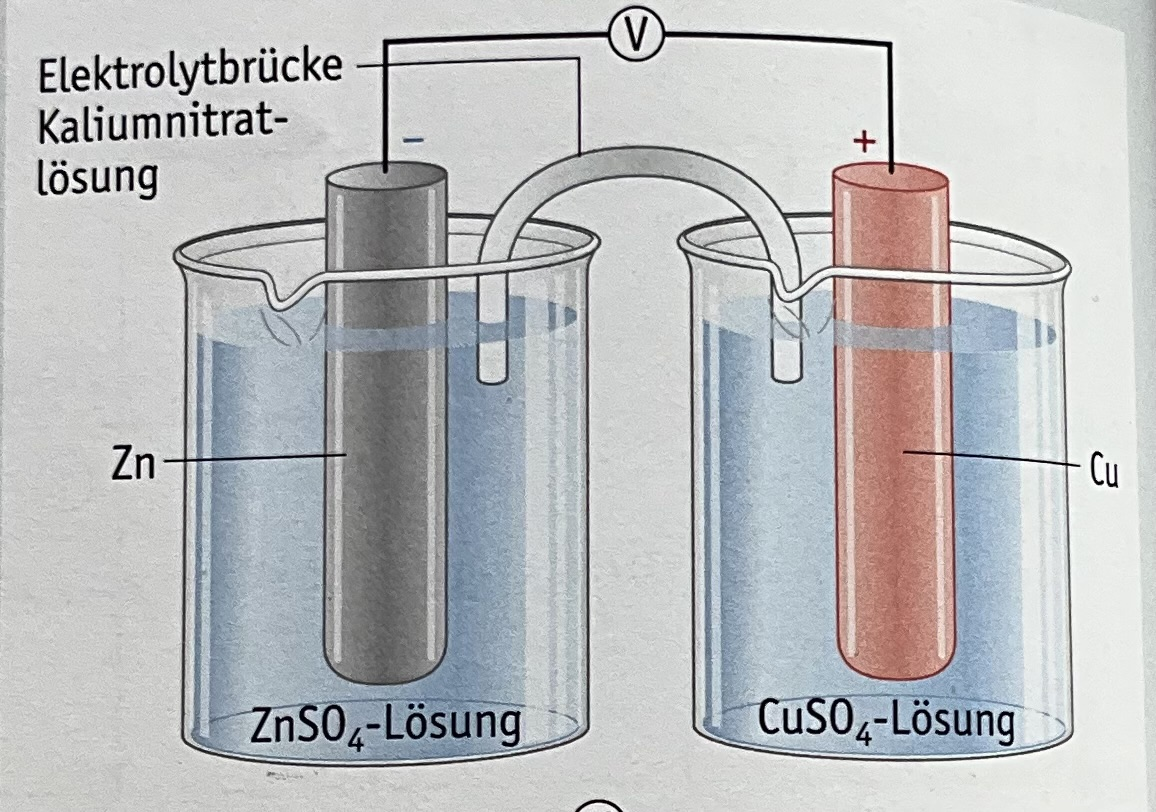
\includegraphics[width=0.5\textwidth]{Bild Protokoll.jpeg}
    \caption*{Ein beispielhafter Versuchsaufbau}
\end{figure*}

\begin{enumerate}
    \item \ce{ZnSO4_{(aq)}}, \ce{CuSO4_{(aq)}}, \ce{AgNO3_{(aq)}} und \ce{FeSO4_{(aq)}} in Bechergläser füllen
    \item Kabel mit Voltmeter verbinden, an den jeweils anderen Enden Krokodilklemmen befestigen
    \item Filterpapier in die \ce{KNO3}-Lösung tunken
    \item für alle Kombinationen an zwei Metallen:
    \begin{enumerate}
        \item Krokodilklemmen an die Bleche klemmen
        \item die Metallbleche in die jeweilige Lösung tunken
        \item beide Lösungen mit dem Filterpapier verbinden (Elektrolytbrücke)
        \item währenddessen die Spannung mit dem Voltmeter messen
    \end{enumerate}
\end{enumerate}

\subsection*{Beobachtung}
\begin{tabular}{|c|c|}
    \hline
    Metallkombination & Gemessene Spannung $U$ \\
    \hline
    \ce{Zn - Cu} &  \\
    \ce{Zn - Ag} &  \\
    \ce{Zn - Fe} &  \\
    \ce{Cu - Ag} &  \\
    \ce{Cu - Fe} &  \\
    \ce{Ag - Fe} &  \\
    \hline
\end{tabular}

\subsection*{Auswertung}
\subsubsection*{Berechnung}
$ U\degree = E\degree(\textrm{Akzeptor}) - E\degree(\textrm{Donator}) $

\begin{tabular}{|c|c|r|l|}
    \hline
    Akzeptor & Donator & Errechnete Spannung $U\degree$ & $U\degree - U = \Delta U$ \\
    \hline
    \ce{ Cu^2+ } & \ce{ Zn^2+ } & $ 0,35 \text{ V} - (-0,76 \text{ V}) = 1,11 \text{ V} $ &  \\
    \ce{ Ag+ }   & \ce{ Zn^2+ } & $ 0,80 \text{ V} - (-0,76 \text{ V}) = 1,56 \text{ V} $ &  \\
    \ce{ Fe^2+ } & \ce{ Zn^2+ } & $ -0,41 \text{ V} - (-0,76 \text{ V}) = 0,35 \text{ V} $ &  \\
    \ce{ Ag+ }   & \ce{ Cu^2+ } & $ 0,80 \text{ V} - 0,35 \text{ V} = 0,45 \text{ V} $ &  \\
    \ce{ Cu^2+ } & \ce{ Fe^2+ } & $ 0,35 \text{ V} - (-0,41 \text{ V}) = 0,76 \text{ V} $ &  \\
    \ce{ Ag+ }   & \ce{ Fe^2+ } & $ 0,80 \text{ V} - (-0,41 \text{ V}) = 1,21 \text{ V} $ &  \\
    \hline
\end{tabular}

\subsubsection*{Reaktionsgleichungen}
\begin{tabular}{|c|l l|c|}
    \hline
    Metallkombination & \multicolumn{2}{|c|}{Teilreaktion} & Gesamtreaktion \\
    \hline
    \multirow{2}{*}{\ce{Zn - Cu}} &
    Ox.: & \ce{ Zn \rightleftarrows Zn^2+ + 2e- } & \multirow{2}{*}{\ce{ Zn + Cu^2+ \rightleftarrows Zn^2+ + Cu }} \\&
    Re.: & \ce{ Cu^2+ + 2e^- \rightleftarrows Cu } &  \\[5pt]
    \multirow{2}{*}{\ce{Zn - Ag}} &
    Ox.: & \ce{ Zn \rightleftarrows Zn^2+ + 2e- } & \multirow{2}{*}{\ce{ Zn + 2Ag+ \rightleftarrows Zn^2+ + 2Ag }} \\&
    Re.: & \ce{ Ag+ + e- \rightleftarrows Ag } &  \\[5pt]
    \multirow{2}{*}{\ce{Zn - Fe}} &
    Ox.: & \ce{ Zn \rightleftarrows Zn^2+ + 2e- } & \multirow{2}{*}{\ce{ Zn + Fe^2+ \rightleftarrows Zn^2+ + Fe }} \\&
    Re.: & \ce{ Fe^2+ + 2e- \rightleftarrows Fe } &  \\[5pt]
    \multirow{2}{*}{\ce{Cu - Ag}} &
    Ox.: & \ce{ Cu \rightleftarrows Cu^2+ + 2e- } & \multirow{2}{*}{\ce{ Cu + 2Ag+ \rightleftarrows Cu^2+ + 2Ag }} \\&
    Re.: & \ce{ Ag+ + e- \rightleftarrows Ag } &  \\[5pt]
    \multirow{2}{*}{\ce{Cu - Fe}} &
    Ox.: & \ce{ Fe \rightleftarrows Fe^2+ + 2e- } & \multirow{2}{*}{\ce{ Fe + Cu^2+ \rightleftarrows Fe^2+ + Cu }} \\&
    Re.: & \ce{ Cu^2+ + 2e- \rightleftarrows Cu } &  \\[5pt]
    \multirow{2}{*}{\ce{Ag - Fe}} &
    Ox.: & \ce{ Fe \rightleftarrows Fe^2+ + 2e- } & \multirow{2}{*}{\ce{ Fe + 2Ag+ \rightleftarrows Fe^2+ + 2Ag }} \\&
    Re.: & \ce{ Ag+ + e- \rightleftarrows Ag } &  \\
    \hline
\end{tabular}

\subsection*{Deutung}
Die gemessenen Spannungen weichen von den errechneten ab. Neben Messunsicherheiten können weitere Ursachen hierfür eine Konzentration des Elektrolyts $\neq 1\textrm{ mol}\cdot\textrm{l}^{-1}$ sowie eine Temperatur $\neq 25 ~\degree\textrm{C}$ sein, da beide Faktoren sich messbar auf die erzeugte Spannung auswirken können.

\end{document}